\documentclass{standalone}
\usepackage{graphicx}	
\usepackage{amssymb, amsmath}
\usepackage{color}

\usepackage{tikz}
\usetikzlibrary{calc, arrows.meta}
\usepackage{pgfmath}

\definecolor{light}{RGB}{220, 188, 188}
\definecolor{mid}{RGB}{185, 124, 124}
\definecolor{dark}{RGB}{143, 39, 39}
\definecolor{highlight}{RGB}{180, 31, 180}
\definecolor{gray10}{gray}{0.1}
\definecolor{gray20}{gray}{0.2}
\definecolor{gray30}{gray}{0.3}
\definecolor{gray40}{gray}{0.4}
\definecolor{gray60}{gray}{0.6}
\definecolor{gray70}{gray}{0.7}
\definecolor{gray80}{gray}{0.8}
\definecolor{gray90}{gray}{0.9}
\definecolor{gray95}{gray}{0.95}

\newcommand*{\offset}{0.025}

\begin{document}

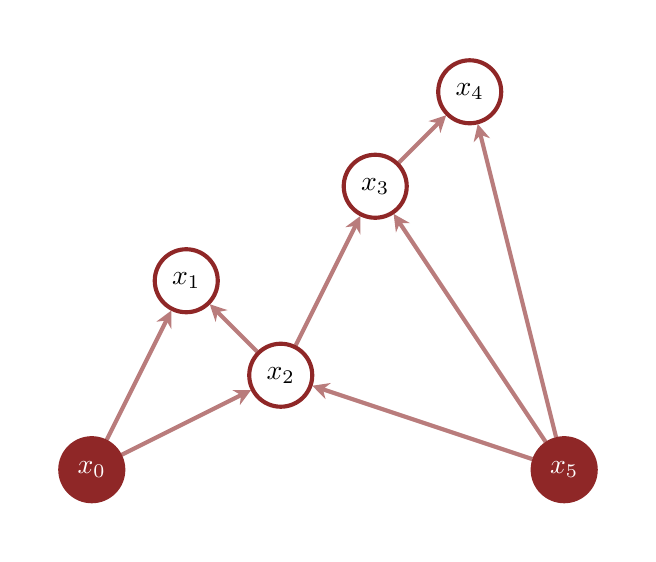
\begin{tikzpicture}[scale=0.2, thick]

  \pgfmathsetmacro{\r}{2}

  \begin{scope}[shift={(0, 0)}]
  
    \draw[white] (-4, -4) rectangle (34, 28);
  
    \coordinate (A) at (0, 0);
    \coordinate (B) at (6, 12);
    \coordinate (C) at (12, 6);
    \coordinate (D) at (18, 18);
    \coordinate (E) at (24, 24);
    \coordinate (F) at (30, 0);
    
    \foreach \B/\E in {A/C, F/C, C/B, A/B, C/D, F/D, D/E, F/E} {
      \draw[-{Stealth[length=6pt, width=6pt]}, shorten <=12.1, shorten >=12, color=mid, line width=1.5] (\B) -- (\E);
    }
    
    \filldraw[fill=dark, draw=dark, line width=1.5] (A) circle (\r)
    node[color=white] { $x_{0}$ };
  
    \filldraw[fill=white, draw=dark, line width=1.5] (B) circle (\r)
    node[color=black] { $x_{1}$ };
  
    \filldraw[fill=white, draw=dark, line width=1.5] (C) circle (\r)
    node[color=black] { $x_{2}$ };
    
    \filldraw[fill=white, draw=dark, line width=1.5] (D) circle (\r)
    node[color=black] { $x_{3}$ };
    
    \filldraw[fill=white, draw=dark, line width=1.5] (E) circle (\r) 
    node[color=black] { $x_{4}$ };
    
    \filldraw[fill=dark, draw=dark, line width=1.5] (F) circle (\r)
    node[color=white] { $x_{5}$ };

  \end{scope}



\end{tikzpicture}

\end{document}  